% 第13章第2节：最小成本（合并本地成本与子消息、消去接口外变量、根袋求值、最优配置的记录与恢复、计算正确性、四环算例与边界检验）。

\section{最小成本}
\label{sec:graph-dp-min-cost}

本节的输入是各变量的有限状态集合、局部成本表（取值于$\mathbb R\cup\{+\infty\}$），以及上一节固定的袋树、根、后序和局部项归属；输出是最小成本$F^\star=\min_{\bm x}F(\bm x)$，并在$F^\star$有限时给出一个达到它的配置，在$F^\star=+\infty$时报告没有可行配置。数值递推、达到值的记录、回溯、正确性与检验在本节一起展开。

\subsection{合并本地成本与子消息}
\label{sec:graph-dp-bag-merge}

处理节点$u$时，它的子节点都已处理完，各自交来一张以接口为索引的消息表$m_{c\to u}(\bm x_{S_c})$，$c\in\operatorname{ch}(u)$。第一步是把本地成本与这些消息按同一个袋配置读取并相加：
\begin{equation}
g_u(\bm x_{B_u})=\Phi_u(\bm x_{B_u})+\sum_{c\in\operatorname{ch}(u)}m_{c\to u}(\bm x_{S_c}).
\label{eq:graph-dp-bag-merge}
\end{equation}
由于$S_c\subseteq B_u$、$S_a\subseteq B_u$（$a\in A_u$），右端每一项都只读取$\bm x_{B_u}$的一部分分量，按第~\ref{sec:graph-dp-root-order}小节的对齐方式取出即可。$g_u$的含义是：袋内变量取定$\bm x_{B_u}$时，$u$本地的成本加上各子节点下方最好能做到的成本。

叶节点没有子消息，求和为空，$g_u=\Phi_u$；没有局部项归入的节点$\Phi_u\equiv0$，$g_u$只由子消息组成。两种空和都取$0$，每项原始成本仍恰好计入一次：它在自己所归的节点计入$\Phi$，此后只以消息的形式向上传递。

在四环算例中，叶节点$\{1,2,4\}$的合并结果是
\[
g(x_1,x_2,x_4)=\phi_{1,2}(x_1,x_2)+\phi_{1,4}(x_1,x_4);
\]
根$\{2,3,4\}$的合并结果是$\phi_{2,3}+\phi_{3,4}$加上叶节点交来的消息。

\subsection{消去接口外变量}
\label{sec:graph-dp-bag-idea}
\label{sec:graph-dp-elimination-idea}

第二步对内部变量取最小。记父节点为$p=p(u)$、接口为$S_u=B_u\cap B_p$，从$u$发往$p$的消息是
\begin{equation}
m_{u\to p}(\bm x_{S_u})=\min_{\bm x_{I_u}}g_u(\bm x_{S_u},\bm x_{I_u}),\qquad I_u=B_u\setminus S_u .
\label{eq:graph-dp-bag-message}
\end{equation}
这与式~\eqref{eq:graph-dp-tree-message}的结构相同，只是被汇总的不再是单个变量，而是袋内全部非接口变量。

可以把每个袋想成一个只看得见袋内变量的计算者。$u$向父节点汇报的是：“若接口取这组值，我这一侧最好能做到多少成本。”父节点不需要知道$u$一侧的其他变量取什么，因为由第~\ref{sec:graph-dp-interface-separation}小节的分隔性质，这些变量不会在父节点一侧再出现，它们只需在$u$一侧选好即可。“$u$一侧最好能做到多少”这一含义在第~\ref{sec:graph-dp-min-cost-correctness}小节证明。

\paragraph{两种退化情形}
接口为空时，消息只有一项，是一个数，但仍须对全部内部配置取最小，不能省去这一步。没有内部变量时（$B_u\subseteq B_p$），式~\eqref{eq:graph-dp-bag-message}中没有可取最小的变量，消息就是$g_u$本身，作为$\bm x_{S_u}=\bm x_{B_u}$的函数原样交给父节点。

\paragraph{数值消元更新}
内部变量只有一个时，式~\eqref{eq:graph-dp-bag-message}就是式~\eqref{eq:graph-dp-elimination-step}的数值消元更新：消元森林中第$i$个袋的内部变量是$v_i$，消息就是$\psi_i$（定理~\ref{thm:graph-dp-elimination-equals-messages}）。

在三元作用域例子中消去$x_1$：只有$\phi_A$含$1$，$S_1=\{2,3\}$。对$(x_2,x_3)=(0,0),(0,1),(1,0),(1,1)$，分别比较$x_1=0,1$两行，得到
\[
\psi_1(x_2,x_3)=\bigl(\min(1,0),\ \min(0,2),\ \min(2,1),\ \min(+\infty,2)\bigr)=(0,\,0,\,1,\,2),
\]
达到最小值的$x_1$依次为$1,0,1,1$。消元后的函数集合是$\{\psi_1,\phi_B\}$。

这一步没有改变剩余变量的最优成本，可以逐项核对。

例如取$(x_2,x_3,x_4)=(1,0,1)$，原问题对$x_1$求最小值为
\[
\begin{aligned}
&\min\bigl(\phi_A(0,1,0)+\phi_B(1,0,1),\ \phi_A(1,1,0)+\phi_B(1,0,1)\bigr)\\
&\qquad=\min(2,1)=1.
\end{aligned}
\]
新集合给出
\[
\psi_1(1,0)+\phi_B(1,0,1)=1+0=1,
\]
两者相同。第~\ref{sec:graph-dp-min-cost-correctness}小节证明这种一致对每个剩余配置、每一步消元都成立。

\subsection{根袋求值}
\label{sec:graph-dp-root-evaluation}

全部非根节点处理完后，根$r$按式~\eqref{eq:graph-dp-bag-merge}合并本地成本与全部子消息，得到$g_r(\bm x_{B_r})$。根的内部变量是整个$B_r$，于是
\begin{equation}
F^\star=\min_{\bm x_{B_r}}g_r(\bm x_{B_r}).
\label{eq:graph-dp-root-min}
\end{equation}
用消元表示时，这对应消去根袋中剩余的变量，剩下的常数就是最小成本。

原始图不连通时，其他分量的根经空接口交来的消息都是标量，即各分量的最小成本；它们作为常数加进$g_r$，所以$F^\star$等于各分量最小成本之和。这与式~\eqref{eq:graph-dp-min-rules}后的第三条规则一致：互不相交的变量组可以分别取最小再相加。

若$F^\star=+\infty$，报告没有可行配置，不做恢复；若$F^\star$有限，进入下一小节的恢复步骤。

\subsection{最优配置的记录与恢复}
\label{sec:graph-dp-min-cost-recovery}
\label{sec:graph-dp-bag-algorithm}
\label{sec:graph-dp-elimination-algorithm}

与链和树上一样，取最小值丢掉了达到者，所以计算消息时要同时记录达到值。对每个接口取值$\bm x_{S_u}$，若$m_{u\to p}(\bm x_{S_u})$有限，记下一个达到最小值的内部取值$b_u(\bm x_{S_u})\in\prod_{i\in I_u}\mathcal X_i$，称为回溯表；并列时按固定规则选取，本部分约定取字典序最小者。若$m_{u\to p}(\bm x_{S_u})=+\infty$，这个接口取值下没有可行的内部取值，不生成记录。根处同样记下$g_r$的一个最小点。

恢复按前序进行：
\begin{itemize}
  \item 根：取$g_r$的最小点（并列时取字典序最小者）作为$\bm x^\star_{B_r}$；
  \item 非根节点：轮到$u$时，它的接口变量都在父袋中，父节点已经处理，所以$\bm x^\star_{S_u}$已经取定；查$b_u(\bm x^\star_{S_u})$，给内部变量$\bm x^\star_{I_u}$赋值。
\end{itemize}
每个变量恰在一个节点作内部变量（引理~\ref{lem:graph-dp-unique-internal}），所以恰被赋值一次，在它出现的所有袋中取同一个值。用消元表示时，按前序恢复就是按消元的逆序回溯：轮到$v_i$时，$S_i$中的变量都比$v_i$晚消去，在逆序中已经取定。

\paragraph{两种表示的算法}
按消元次序直接计算时，每个函数存为一个作用域和一张稠密表，并为每个变量维护一张索引，列出当前作用域含它的函数，消去$x_i$时据此直接取出$\mathcal F_i$，不必扫描全部函数。算法维护当前函数集合（初值为全部局部函数）、已消去的变量集合和各步的回溯表。

\begin{algorithm}[变量消元求最小成本]
\label{alg:graph-dp-variable-elimination}
输入：有限状态集合、局部函数表、一个消元次序。输出：最小成本，以及一个最优配置或“不可行”。
\begin{enumerate}
  \item 按次序取下一个变量$x_i$，由变量索引取出当前全部含$i$的函数$\mathcal F_i$，确定$S_i$。
  \item 对$\bm x_{S_i}$的每个取值，枚举$x_i$的全部状态，按式~\eqref{eq:graph-dp-elimination-step}求$\psi_i$；同时把达到最小值的$x_i$（并列时取编号最小者）记入回溯表$b_i(\bm x_{S_i})$。
  \item 用$\psi_i$替换$\mathcal F_i$，同步更新$S_i$中各变量的索引；重复直到变量全部消去，剩下的常数之和即最小成本。
  \item 若最小成本为$+\infty$，报告不可行；否则按消元的逆序依次令$x_i=b_i(\bm x_{S_i})$。
\end{enumerate}
\end{algorithm}

\begin{algorithm}[树分解上的最小成本动态规划]
\label{alg:graph-dp-bag-dp}
输入：局部函数表，原始图的已核验树分解。输出：最小成本，以及一个最优配置或“不可行”。
\begin{enumerate}
  \item 把每个局部函数归入一个包含其作用域的袋，按式~\eqref{eq:graph-dp-bag-cost}计算各袋本地成本$\Phi_u$。
  \item 选根节点$r$，求出每个节点的父节点、接口、内部变量和一个后序。
  \item 按后序处理每个非根节点$u$：按式~\eqref{eq:graph-dp-bag-merge}合并得$g_u$；对接口$S_u$的每种取值，枚举$I_u$的全部取值，按式~\eqref{eq:graph-dp-bag-message}计算$m_{u\to p(u)}$，并把达到最小值的内部取值记入$b_u$。
  \item 合并得$g_r$，按式~\eqref{eq:graph-dp-root-min}计算最小成本；若为$+\infty$，报告不可行并停止。
  \item 取$g_r$的最小点为根袋变量赋值；按前序处理每个非根节点$u$，查$b_u$为$I_u$赋值。
\end{enumerate}
\end{algorithm}

\paragraph{消元的执行过程}
在三元作用域例子上按次序$(1,4,2,3)$执行算法~\ref{alg:graph-dp-variable-elimination}。下面逐步比较更新前后的函数集合，最后用表~\ref{tab:graph-dp-elimination-trace}汇总数值。

消去$x_1$：如上一小节，$\mathcal F_1=\{\phi_A\}$，$S_1=\{2,3\}$，$\psi_1=(0,0,1,2)$，$b_1=(1,0,1,1)$。函数集合变为$\{\psi_1,\phi_B\}$。
\begin{BookInlineFigure}
  \centering
  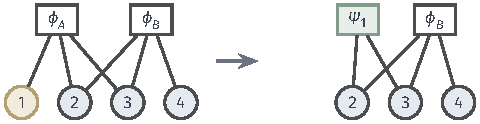
\includegraphics[width=81.284mm]{figures/03-graphs/04-local-functions-and-dynamic-programming/tikz/reading-steps/eliminate-x1.pdf}
  \caption{消去$x_1$：把读取它的$\phi_A$替换为$\psi_1(x_2,x_3)$，$\phi_B$不变。圆点为变量，方块为函数，连线表示读取关系；左侧黄色变量被汇总，右侧绿色方块是新函数。}
  \label{fig:graph-dp-elimination-trace}
\end{BookInlineFigure}

消去$x_4$：只有$\phi_B$含$4$，$S_4=\{2,3\}$。对$(x_2,x_3)$的四种取值比较$x_4=0,1$，得到
  \[
  \psi_4=\bigl(\min(2,1),\ \min(0,+\infty),\ \min(+\infty,0),\ \min(1,2)\bigr)=(1,0,0,1),
  \]
  回溯表$b_4=(1,0,1,0)$。函数集合变为$\{\psi_1,\psi_4\}$。
\begin{BookInlineFigure}
  \centering
  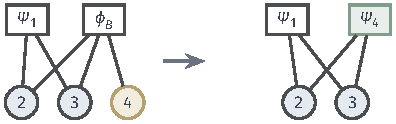
\includegraphics[width=67.035mm]{figures/03-graphs/04-local-functions-and-dynamic-programming/tikz/reading-steps/eliminate-x4.pdf}
  \caption{消去$x_4$：$\phi_B$被$\psi_4(x_2,x_3)$替换。此时两个函数只共享接口变量$x_2,x_3$。}
  \label{fig:graph-dp-elimination-trace-x4}
\end{BookInlineFigure}

消去$x_2$：$\psi_1$和$\psi_4$都含$2$，要先相加再对$x_2$取最小，$S_2=\{3\}$。$x_3=0$时两个候选为
  \[
  \psi_1(0,0)+\psi_4(0,0)=1,\qquad \psi_1(1,0)+\psi_4(1,0)=1,
  \]
  二者并列，按约定取$x_2=0$。$x_3=1$时候选为$0+0=0$与$2+1=3$，取$x_2=0$。新函数记为$\psi_2'=(1,0)$，以区别于第~\ref{sec:graph-dp-fill-in}小节先消$x_2$时的$\psi_2$；$b_2=(0,0)$。
\begin{BookInlineFigure}
  \centering
  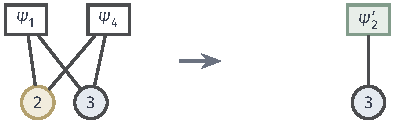
\includegraphics[width=66.784mm]{figures/03-graphs/04-local-functions-and-dynamic-programming/tikz/reading-steps/eliminate-x2.pdf}
  \caption{消去$x_2$：先把同一$(x_2,x_3)$下的$\psi_1$与$\psi_4$相加，再对$x_2$取最小。两项共同被一元函数$\psi_2'(x_3)$替换。}
  \label{fig:graph-dp-elimination-trace-x2}
\end{BookInlineFigure}

消去$x_3$：只剩$\psi_2'$，$S_3=\varnothing$，$\min(1,0)=0$在$x_3=1$处达到，$b_3=1$。函数集合只剩常数$0$，即最小成本。
\begin{BookInlineFigure}
  \centering
  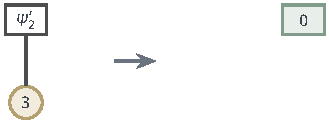
\includegraphics[width=55.785mm]{figures/03-graphs/04-local-functions-and-dynamic-programming/tikz/reading-steps/eliminate-x3.pdf}
  \caption{消去$x_3$：对最后的一元函数$\psi_2'$取最小，得到常数$0$。新函数已无变量，因而右侧没有连线。}
  \label{fig:graph-dp-elimination-trace-x3}
\end{BookInlineFigure}

最小成本有限，按逆序$3,2,4,1$回溯：
\[
\begin{gathered}
x_3=b_3=1,\qquad x_2=b_2(x_3{=}1)=0,\\
x_4=b_4(x_2{=}0,x_3{=}1)=0,\qquad x_1=b_1(x_2{=}0,x_3{=}1)=0.
\end{gathered}
\]

\begin{BookInlineFigure}
  \centering
  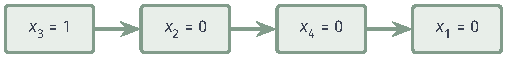
\includegraphics[width=85.785mm]{figures/03-graphs/04-local-functions-and-dynamic-programming/tikz/reading-steps/elimination-recovery.pdf}
  \caption{按消元的逆序查回溯表。先确定$x_3$，再用已知接口值依次读取$b_2,b_4,b_1$，恢复$(x_1,x_2,x_3,x_4)=(0,0,1,0)$。}
  \label{fig:graph-dp-elimination-trace-recovery}
\end{BookInlineFigure}

恢复的配置为$(0,0,1,0)$，代回表~\ref{tab:graph-dp-ternary-tables}得
\[
\phi_A(0,0,1)+\phi_B(0,1,0)=0+0=0,
\]
与枚举结果一致。

\begin{table}[!htb]
  \centering
  \small
  \begin{tabular}{@{}cccccc@{}}
    \toprule
    消去 & 取出$\mathcal F_i$ & $S_i$ & 新函数$\psi_i$ & 回溯表$b_i$ & 消元后的$\mathcal F$\\
    \midrule
    $x_1$ & $\phi_A$ & $\{2,3\}$ & $(0,0,1,2)$ & $(1,0,1,1)$ & $\{\psi_1,\phi_B\}$\\
    $x_4$ & $\phi_B$ & $\{2,3\}$ & $(1,0,0,1)$ & $(1,0,1,0)$ & $\{\psi_1,\psi_4\}$\\
    $x_2$ & $\psi_1,\psi_4$ & $\{3\}$ & $(1,0)$ & $(0,0)$ & $\{\psi_2'\}$\\
    $x_3$ & $\psi_2'$ & $\varnothing$ & $0$ & $1$ & $\{0\}$\\
    \bottomrule
  \end{tabular}
  \caption{按次序$(1,4,2,3)$对三元作用域例子消元。新函数与回溯表的取值按剩余变量的字典序列出：作用域为$\{2,3\}$时依次对应$(x_2,x_3)=(0,0),(0,1),(1,0),(1,1)$，作用域为$\{3\}$时对应$x_3=0,1$。}
  \label{tab:graph-dp-elimination-trace}
\end{table}


\paragraph{袋树上的执行过程}
同一个例子也可以直接在两个袋$B_s=\{1,2,3\}$、$B_t=\{2,3,4\}$上执行算法~\ref{alg:graph-dp-bag-dp}，取$t$为根，后序为$s,t$。本地成本为$\Phi_s=\phi_A$、$\Phi_t=\phi_B$。

$s$是叶节点，没有子消息，内部变量只有$x_1$，所以
\[
m_{s\to t}(x_2,x_3)=\min_{x_1}\phi_A(x_1,x_2,x_3).
\]
图~\ref{fig:graph-dp-bag-message-table}逐行列出了这张四项表：接口取值为$00,01,10,11$时，消息值依次为$0,0,1,2$，达到最小值的$x_1$依次为$1,0,1,1$。它与消去$x_1$得到的$\psi_1$相同。

$x_1$已经被汇总，不再出现在表中；$x_2,x_3$作为接口仍然显式保留，根袋读取这张表时要按同样的$(x_2,x_3)$取值对齐。

根处合并得$g_t=\phi_B+m_{s\to t}$，按$(x_2,x_3,x_4)$的字典序依次为
\[
g_t=(2,\,1,\,0,\,+\infty,\,+\infty,\,1,\,3,\,4),
\]
最小值$0$在$(0,1,0)$处达到。

回溯时根取$(x_2,x_3,x_4)=(0,1,0)$，查叶节点的回溯表得$b_s(0,1)=0$，即$x_1=0$。恢复的配置$(0,0,1,0)$与枚举和消元的结果相同。

\begin{figure}[!htb]
  \centering
  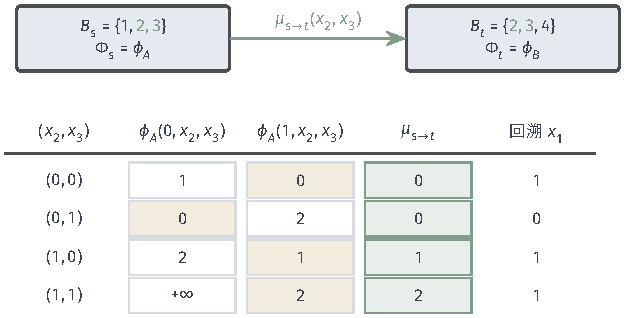
\includegraphics[width=105.650mm]{figures/01-basic-mathematics/04-graphs/tikz/c5-bag-message-table/figure.pdf}
  \caption{两袋之间的消息。左袋$B_s=\{1,2,3\}$只含$\phi_A$，右袋$B_t=\{2,3,4\}$只含$\phi_B$，接口为$\{2,3\}$（绿色）。下方表格对接口的每种取值比较$x_1=0,1$两个候选，取较小者作为消息值，黄色格是被选中的候选；绿色列是消息值，最后一列是回溯表。根袋$B_t$把消息与$\phi_B$相加后对$x_2,x_3,x_4$取最小，得到最优值$0$。}
  \label{fig:graph-dp-bag-message-table}
\end{figure}

\subsection{计算正确性}
\label{sec:graph-dp-min-cost-correctness}
\label{sec:graph-dp-bag-analysis}
\label{sec:graph-dp-elimination-analysis}

\paragraph{消息的不变量}
正确性归结为一个不变量：每条消息等于固定接口后，下方全部局部项之和的最小值。对非根节点$u$，记$D_u$为$u$及其全部后代组成的节点集合，$V_{D_u}=\bigcup_{t\in D_u}B_t$为这些袋中出现的变量，$A_{D_u}=\bigcup_{t\in D_u}A_t$为归入这些节点的局部项。

\begin{theorem}[袋消息的含义]
\label{thm:graph-dp-bag-message}
设$(\mathcal T,\{B_t\}_{t\in T})$是原始图的树分解，以$r$为根，每个局部函数恰好归入一个包含其作用域的袋。则对每个非根节点$u$和每个接口取值$\bm x_{S_u}$，
\[
m_{u\to p(u)}(\bm x_{S_u})=\min_{\bm x_{V_{D_u}\setminus S_u}}\ \sum_{a\in A_{D_u}}\phi_a(\bm x_{S_a}).
\]
进一步，$\min_{\bm x}F(\bm x)=\min_{\bm x_{B_r}}g_r(\bm x_{B_r})$。
\end{theorem}

\begin{proof}
对$|D_u|$归纳，叶节点是起点。设$u$的子节点为$c_1,\ldots,c_k$（叶节点时$k=0$）。$D_u$由$u$和各$D_{c_j}$组成，于是$A_{D_u}$分为$A_u$和各$A_{D_{c_j}}$，每个局部项恰在一处。

先看变量怎样分开。由引理~\ref{lem:graph-dp-interface-separation}应用于袋树边$\{c_j,u\}$，$V_{D_{c_j}}$与$D_{c_j}$以外各袋的公共变量都在$S_{c_j}\subseteq B_u$中。所以集合
\[
I_u,\qquad V_{D_{c_1}}\setminus B_u,\qquad\ldots,\qquad V_{D_{c_k}}\setminus B_u
\]
两两不交：$V_{D_{c_j}}\setminus B_u$中的变量不在$B_u$里，也不在其他子树中。它们的并恰为$V_{D_u}\setminus S_u$。另一方面，$A_{D_{c_j}}$中函数的变量都在$V_{D_{c_j}}$中，其中属于$B_u$的部分又在$S_{c_j}$中。

现在固定$\bm x_{B_u}$。各$A_{D_{c_j}}$中函数之和只依赖$\bm x_{S_{c_j}}$与互不相交的变量组$\bm x_{V_{D_{c_j}}\setminus B_u}$，按式~\eqref{eq:graph-dp-min-rules}后的第三条规则可以分别求最小；由归纳假设，第$j$项的最小值为$m_{c_j\to u}(\bm x_{S_{c_j}})$。归入$u$的局部项与这些变量无关，由第二条规则留在最小化之外。于是固定$\bm x_{B_u}$后的最小值是$g_u(\bm x_{B_u})$。再对$\bm x_{I_u}$求最小值，由第一条规则，就得到式~\eqref{eq:graph-dp-bag-message}。

根处的等式用同样的拆分得到：由顶点覆盖，全部变量是$B_r$与各$V_{D_c}\setminus B_r$（$c\in\operatorname{ch}(r)$）的不交并，全部局部项分为归入$r$的与归入各子树的。
\end{proof}

证明用到了三项条件：运行交集保证接口隔开两侧；顶点覆盖保证根处的汇总涉及全部变量；每个局部函数恰好归入一个容纳它的袋，保证每一项只计一次。少了任何一项，递推得到的数都可能不等于原问题的最小值。

\paragraph{任意消元次序都正确}
按消元次序直接计算时，正确性也可以用一个不变量表述，并且它对任意次序都成立。设已经按某个次序消去了下标集合$Z$中的变量，把剩余变量的一个配置记为$\bm y=\bm x_{V\setminus Z}$。消元过程保持
\begin{equation}
\sum_{f\in\mathcal F}f(\bm y)=\min_{\bm x_Z}F(\bm x_Z,\bm y)\qquad\text{对每个剩余配置}\ \bm y .
\label{eq:graph-dp-elimination-invariant}
\end{equation}

\begin{theorem}[变量消元的正确性]
\label{thm:graph-dp-elimination}
设各变量的状态集合有限，总成本由式~\eqref{eq:graph-dp-local-sum}给出。从$\mathcal F=\{\phi_a:a\in A\}$出发，按任意次序反复执行式~\eqref{eq:graph-dp-elimination-step}的消元操作，则每一步之后不变量~\eqref{eq:graph-dp-elimination-invariant}都成立。特别地，消去全部变量后剩下的常数之和等于$\min_{\bm x}F(\bm x)$；只消去$V\setminus R$中的变量时，剩余函数之和是关于$\bm x_R$的表，在每个$\bm x_R$处等于$\min_{\bm x_{V\setminus R}}F(\bm x)$。
\end{theorem}

\begin{proof}
开始时$Z=\varnothing$，当前函数之和就是$F$，不变量成立。设消去$x_i$之前不变量对$Z$成立。把当前函数分为含$i$的$\mathcal F_i$与其余部分$\mathcal F_{-i}$。固定$Z\cup\{i\}$以外的变量后，$\mathcal F_{-i}$中各函数的值与$x_i$无关，按式~\eqref{eq:graph-dp-min-rules}可以移出对$x_i$的最小化：
\[
\min_{x_i}\Bigl[\sum_{f\in\mathcal F_{-i}}f+\sum_{f\in\mathcal F_i}f\Bigr]
=\sum_{f\in\mathcal F_{-i}}f+\min_{x_i}\sum_{f\in\mathcal F_i}f
=\sum_{f\in\mathcal F_{-i}}f+\psi_i .
\]
右端正是消元后的函数之和。左端由不变量等于$\min_{x_i}\min_{\bm x_Z}F$，再由式~\eqref{eq:graph-dp-min-rules}的第一条等于$\min_{\bm x_{Z\cup\{i\}}}F$。所以不变量对$Z\cup\{i\}$成立。对消元步数归纳即得结论。
\end{proof}

这个定理说明，纯最小化中改变消元次序不改变最小值，但中间表与计算代价可以变化。三元作用域例子按次序$(2,1,3,4)$消元时，第一步得到第~\ref{sec:graph-dp-fill-in}小节的$8$项表$\psi_2$，其后依次得到$(x_3,x_4)$上的$(2,1,0,4)$、$x_4$上的$(0,1)$和常数$0$，逆序回溯同样恢复出$(0,0,1,0)$。两种次序得到相同的最小值，而最大中间表分别有$4$项和$8$项（表~\ref{tab:graph-dp-elimination-orders}）。

\paragraph{恢复的配置达到最小值}
回溯给出一致的配置：每个变量恰被赋值一次，接口变量在子节点中沿用父节点已取的值。再对$|D_u|$归纳可知，给定接口取值$\bm x^\star_{S_u}$且$m_{u\to p(u)}(\bm x^\star_{S_u})$有限时，按回溯表给$V_{D_u}\setminus S_u$赋值后，$A_{D_u}$中局部项之和恰好等于$m_{u\to p(u)}(\bm x^\star_{S_u})$。这是因为$b_u$选的内部取值达到式~\eqref{eq:graph-dp-bag-message}的最小值，使$g_u$等于消息；$g_u$中的每条子消息又由归纳假设被子树中的赋值达到，而且这些子消息有限，回溯表中有相应的记录。

在根处，所选的$\bm x^\star_{B_r}$使$g_r$等于$F^\star$，于是整个配置的成本等于$F^\star$。若$F^\star=+\infty$，任何配置都“达到”它，所以算法报告没有可行配置，而不把回溯结果当作最优解输出。逆序回溯的正确性是同一论证在消元森林上的特例；若只保存$\psi_i$而不保存回溯表，就无法直接恢复配置。

回溯表只恢复一个最优配置。若要列出全部并列最优的配置，需要在每个接口取值下记录全部最优的内部取值，而这类配置的数目本身可能随$n$指数增长。

\subsection{四环算例与边界检验}
\label{sec:graph-dp-four-cycle-min}

\paragraph{四环算例}
在四环算例的分解$\{1,2,4\}-\{2,3,4\}$上执行算法~\ref{alg:graph-dp-bag-dp}，以$\{2,3,4\}$为根。归属与第~\ref{sec:graph-dp-term-assignment}小节相同。

叶节点的接口为$\{2,4\}$，内部变量为$\{1\}$。对接口的每种取值比较$x_1=0,1$两个候选$\phi_{1,2}+\phi_{1,4}$，表~\ref{tab:graph-dp-four-cycle-min-messages}的左半部分列出了结果，消息与第~\ref{sec:graph-dp-four-cycle}小节的$\psi_1$相同。

根处合并
\[
g=\phi_{2,3}(x_2,x_3)+\phi_{3,4}(x_3,x_4)+m(x_2,x_4),
\]
表的右半部分按$(x_2,x_3,x_4)$的字典序列出。最小值$3$在$(0,0,1)$处唯一达到。

回溯时根取$(x_2,x_3,x_4)=(0,0,1)$，查叶节点的回溯表得$b(0,1)=1$，恢复$\bm x^\star=(1,0,0,1)$。这与表~\ref{tab:graph-dp-four-cycle-enumeration}的枚举结果一致；代回四项成本$1+1+1+0=3$，每项恰计一次。

\begin{table}[!htb]
  \centering
  \small
  \begin{tabular}{@{}cccc@{\qquad}cc@{}}
    \toprule
    $(x_2,x_4)$ & 候选 & $m$ & $b$ & $(x_2,x_3,x_4)$ & $g$\\
    \midrule
    $(0,0)$ & $6,\ 4$ & $4$ & $1$ & $(0,0,0)$, $(0,0,1)$ & $5$, $3$\\
    $(0,1)$ & $+\infty,\ 1$ & $1$ & $1$ & $(0,1,0)$, $(0,1,1)$ & $7$, $+\infty$\\
    $(1,0)$ & $3,\ 5$ & $3$ & $0$ & $(1,0,0)$, $(1,0,1)$ & $4$, $4$\\
    $(1,1)$ & $+\infty,\ 2$ & $2$ & $1$ & $(1,1,0)$, $(1,1,1)$ & $4$, $+\infty$\\
    \bottomrule
  \end{tabular}
  \caption{四环算例的最小成本计算。左：叶节点$\{1,2,4\}$对$x_1=0,1$的两个候选、消息值与回溯表。右：根$\{2,3,4\}$的合并值$g=\phi_{2,3}+\phi_{3,4}+m$。}
  \label{tab:graph-dp-four-cycle-min-messages}
\end{table}

改用未合并的消元森林，即按次序$(1,2,3,4)$执行算法~\ref{alg:graph-dp-variable-elimination}，第一步同样得到$\psi_1$。消去$x_2$时取出$\psi_1$与$\phi_{2,3}$，得
\[
\psi_2(x_3,x_4)=(4,2,4,3),
\]
回溯表为$(1,0,1,1)$。

消去$x_3$时取出$\psi_2$与$\phi_{3,4}$。$x_4=0$时两个候选$4+0$与$4+0$并列，按约定取$x_3=0$；$x_4=1$时候选为$2+1$与$3+\infty$。于是
\[
\psi_3(x_4)=(4,3).
\]
最后消去$x_4$得常数$3$。逆序回溯给出$x_4=1$、$x_3=0$、$x_2=0$、$x_1=1$，结果相同，中间表则与合并袋上的计算不同。

\paragraph{并列最优}
把$\phi_{2,3}(1,0)$从$1$改为$0$，其余不变。这时$(0,1,0,0)$、$(1,0,0,1)$、$(1,1,0,1)$三个配置的成本都是$3$。叶节点的消息不变，根处$g$在$(0,0,1)$、$(1,0,0)$、$(1,0,1)$三处取最小值$3$。按字典序规则，根取$(0,0,1)$，恢复的仍是$(1,0,0,1)$；若规则改为取字典序最大者，根取$(1,0,1)$，恢复$(1,1,0,1)$。两者都是最优配置，固定规则只是让输出可以复现；要得到全部最优配置，须保留全部达到值。

\paragraph{不可行}
把四项成本换成约束：$\phi_{1,2},\phi_{2,3},\phi_{3,4}$在两端相等时为$0$、不等时为$+\infty$，$\phi_{1,4}$在两端不等时为$0$、相等时为$+\infty$。每张表单独看都有可行的组合，但沿环要求$x_1=x_2=x_3=x_4$且$x_1\neq x_4$，互相矛盾。

叶节点的消息为
\[
m(x_2,x_4)=(+\infty,0,0,+\infty),
\]
即只有$x_2\neq x_4$时存在可行的$x_1$。根处$\phi_{2,3}+\phi_{3,4}$要求$x_2=x_3=x_4$，此时$m=+\infty$，所以$g$的八项全是$+\infty$，算法报告不可行，不做恢复。$+\infty$按运算约定沿消息传递，不需要特殊处理。

\paragraph{孤立变量与多个分量}
在原问题上再加两个分量：一个没有任何局部项的孤立变量$x_5\in\{0,1,2\}$，以及一条边$\{6,7\}$上的成本$\phi_{6,7}$，其表的行对应$x_6$、列对应$x_7$：
\[
\phi_{6,7}=\begin{bmatrix}2&1\\0&3\end{bmatrix}.
\]
结构上增加袋$\{5\}$和$\{6,7\}$，各用一条空接口的边连到根$\{2,3,4\}$。

袋$\{5\}$没有局部项，$g\equiv0$，对三个状态取最小得标量消息$0$，回溯记录$x_5=0$（字典序最小）。袋$\{6,7\}$的接口也为空，消息是$\min\phi_{6,7}=0$，在$(x_6,x_7)=(1,0)$处达到。

根把这两个标量加进$g$，最小成本为$3+0+0=3$，恢复的配置在原四个变量上不变，并有$x_5=0$、$(x_6,x_7)=(1,0)$。孤立变量虽不影响最小值，仍须出现在某个袋中，才会在恢复时被赋值。
